% deep_dive.tex — Quantum vs Classical Pricing on n=20 PSPs
% Adapted from RF-branching/slides/qcg_vs_cg_demo/qcg_vs_cg_demo.tex onto the
% canonical QCi beamer template (~/Code/slide-templates/beamer-qci/).
%
% Compile: pdflatex deep_dive.tex (twice for frame numbers)
\documentclass[aspectratio=169,11pt]{beamer}

% =============================================================
% Theme
% =============================================================
\usetheme{Madrid}
\setbeamertemplate{navigation symbols}{}

% =============================================================
% QCi Brand Colors (from beamer-qci template)
% =============================================================
\usepackage[table]{xcolor}

\definecolor{QCIcol1}{HTML}{211D53}   % primary dark purple-blue
\definecolor{QCIcol2}{HTML}{908FA8}   % muted gray-purple
\definecolor{QCIcol3}{HTML}{D3DAE6}   % light blue-gray (block bg)
\definecolor{QCIcol4}{HTML}{E8ECF2}   % pale blue
\definecolor{QCIcol5}{HTML}{F6F7FA}   % near-white (slide body bg)
\definecolor{qciorange}{RGB}{220,120,20}
\definecolor{qcigreen}{RGB}{40,140,60}

% Source-deck accent colors (preserved for content-level macros)
\definecolor{qciblue}{RGB}{0,70,130}
\definecolor{qciteal}{RGB}{0,128,128}

% =============================================================
% Beamer Colors
% =============================================================
\setbeamercolor{palette primary}   {bg=QCIcol1,           fg=white}
\setbeamercolor{palette secondary} {bg=QCIcol2,           fg=white}
\setbeamercolor{palette tertiary}  {bg=QCIcol1!70,        fg=white}
\setbeamercolor{palette quaternary}{bg=QCIcol1,           fg=white}
\setbeamercolor{structure}         {fg=QCIcol1}
\setbeamercolor{block title}       {bg=QCIcol3,           fg=QCIcol1}
\setbeamercolor{block body}        {bg=QCIcol5}
\setbeamercolor{block title alerted}{bg=qciorange!20,     fg=qciorange!70!black}
\setbeamercolor{block body alerted} {bg=qciorange!5}
\setbeamercolor{block title example}{bg=qcigreen!15,      fg=qcigreen!70!black}
\setbeamercolor{block body example} {bg=qcigreen!5}
\setbeamercolor{alerted text}      {fg=qciorange}
\setbeamercolor{example text}      {fg=qcigreen!70!black}
\setbeamercolor{section in toc}    {fg=QCIcol1}
\setbeamercolor{subsection in toc} {fg=QCIcol2}
\setbeamercolor{frametitle}        {fg=white}

% =============================================================
% Font  (Raleway — matches qci2.cls)
% =============================================================
\usepackage{anyfontsize}
\usepackage[oldstyle,default]{raleway}
\usefonttheme{default}

% =============================================================
% Packages
% =============================================================
\usepackage{amsmath,amssymb}
\usepackage{booktabs}
\usepackage{array}
\usepackage{colortbl}
\usepackage{graphicx}
\usepackage{tikz}
\usetikzlibrary{calc,positioning,arrows.meta,decorations.pathreplacing,
                shapes.geometric,fit,backgrounds,patterns}

% =============================================================
% Custom Headline (Madrid nav + white logo on right)
% =============================================================
\setbeamertemplate{headline}{%
  \leavevmode%
  \hbox{%
    \begin{beamercolorbox}[wd=.80\paperwidth,ht=2.5ex,dp=1.125ex]{palette primary}%
      \insertsectionnavigationhorizontal{.80\paperwidth}{\hskip0pt plus1filll}{}%
    \end{beamercolorbox}%
    \begin{beamercolorbox}[wd=.20\paperwidth,ht=2.5ex,dp=1.125ex,right]{palette primary}%
      \raisebox{-0.5ex}{
\includegraphics[height=2.5ex]{QCILogoWhite}}\hspace*{6pt}%
    \end{beamercolorbox}}%
}

% =============================================================
% Custom Footline (author | title | frame/total)
% =============================================================
\setbeamertemplate{footline}{%
  \leavevmode\hbox{%
    \begin{beamercolorbox}[wd=.33\paperwidth,ht=2.5ex,dp=1ex,center]{author in head/foot}%
      \usebeamerfont{author in head/foot}\insertshortauthor
    \end{beamercolorbox}%
    \begin{beamercolorbox}[wd=.34\paperwidth,ht=2.5ex,dp=1ex,center]{title in head/foot}%
      \usebeamerfont{title in head/foot}\insertshorttitle
    \end{beamercolorbox}%
    \begin{beamercolorbox}[wd=.33\paperwidth,ht=2.5ex,dp=1ex,right]{date in head/foot}%
      \usebeamerfont{date in head/foot}\insertframenumber{}/\inserttotalframenumber\hspace*{2ex}
    \end{beamercolorbox}}%
}

% =============================================================
% Custom Title Page (mirrors beamer-qci template)
% =============================================================
\setbeamertemplate{title page}{%
  \begin{tikzpicture}[remember picture, overlay, inner sep=0pt]
    \fill[QCIcol5] (current page.south west) rectangle (current page.north east);
    \node[anchor=north] at ([yshift=-0.9cm]current page.north)
      {
\includegraphics[width=3.4cm]{QCIlogo2}};
    \node[QCIcol1, align=center,
          font=\fontsize{9pt}{11pt}\fontseries{sb}\selectfont]
      at ([yshift=1.1cm]current page.south)
      {Quantum Computing Inc\quad|\quad
       quantumcomputinginc.com\quad|\quad
       (703)~436-2161};
  \end{tikzpicture}
  \vspace{2.6cm}
  \begin{center}
    {\usebeamerfont{title}\usebeamercolor[fg]{title}\color{QCIcol1}\inserttitle\par}
    \ifx\insertsubtitle\empty\else
      \vspace{0.3em}
      {\usebeamerfont{subtitle}\color{QCIcol2}\insertsubtitle\par}
    \fi
    \vspace{0.6em}
    {\usebeamerfont{author}\color{QCIcol1}\insertauthor\par}
    \ifx\insertinstitute\empty\else
      \vspace{0.15em}
      {\usebeamerfont{institute}\color{QCIcol2}\insertinstitute\par}
    \fi
    \vspace{0.3em}
    {\usebeamerfont{date}\color{QCIcol2}\insertdate\par}
  \end{center}
}

% =============================================================
% Content macros (preserved from source deck)
% =============================================================
\newcommand{\cmark}{\textcolor{qcigreen}{\checkmark}}
\newcommand{\xmark}{\textcolor{red}{$\times$}}
\newcommand{\bestval}[1]{\textbf{\textcolor{qciteal}{#1}}}
\newcommand{\lpname}{\textcolor{qciblue}{LP pricing}}
\newcommand{\diracname}{\textcolor{qciorange}{Dirac pricing}}

% =============================================================
% Presentation Metadata
% =============================================================
\title[QCG Deep Dive]{Quantum vs Classical Pricing for Column Generation}
\subtitle{Per-PSP comparison on n\,=\,20 Erd\H{o}s--R\'enyi graphs}
\author[QCi Research]{QCi Research}
\institute[QCi]{Quantum Computing Inc}
\date{\today}

\begin{document}

\begin{frame}[plain]
  \titlepage
\end{frame}

\begin{frame}{Outline}
  \tableofcontents
\end{frame}

% ===========================================================================
\section{Problem setup}

\begin{frame}{Graph coloring}
  \textbf{Minimum Vertex Coloring.} Assign colors to vertices so that adjacent
  vertices differ, using as few colors as possible. $\chi(G)$ is the chromatic
  number.
  \begin{itemize}
    \item NP-hard in general; equivalent to partitioning $V$ into independent sets.
    \item Each color class is an \alert{independent set} (IS) of $G$.
  \end{itemize}

  \vspace{0.3em}
  \begin{block}{IS-partition view}
    Minimum coloring $=$ minimum number of ISs that cover $V$. This is a
    \bestval{set-cover} ILP whose columns are the ISs of $G$.
  \end{block}
\end{frame}

\begin{frame}{Our running instance: ER(20, 0.7, seed=0)}
  \begin{center}
    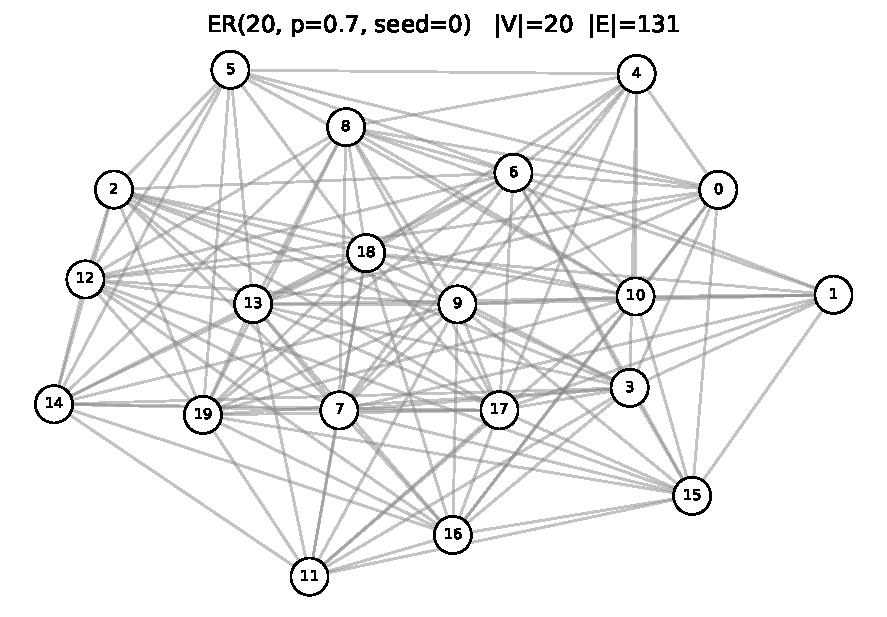
\includegraphics[width=0.78\textwidth]{figures/01_master_graph.pdf}
  \end{center}
  \small $\chi = 8$ (proved by MILP/Hexaly at seconds scale). 131 edges; density $\approx$ 0.69.
\end{frame}

% ===========================================================================
\section{Column generation}

\begin{frame}{Column generation in one page}
  \begin{columns}[T]
    \begin{column}{0.55\textwidth}
      Master LP (relaxation):
      \[
      \min_{y \ge 0} \sum_{S \in \mathcal{S}} y_S
      \quad \text{s.t.} \quad
      \sum_{S \ni v} y_S \ge 1 \ \forall v.
      \]
      $\mathcal{S}$ = all ISs of $G$ is exponential; start with a small subset
      and \alert{generate columns as needed}.
      \vspace{0.5em}

      Pricing subproblem (\textbf{PSP}) at dual $y_v$:
      \[
      \max_{S \text{ IS}} \sum_{v \in S} y_v \;-\; 1
      \quad \text{(negative reduced cost)}
      \]
      Any $S$ with $\sum_v y_v > 1$ is profitable.
    \end{column}
    \begin{column}{0.45\textwidth}
      \centering
      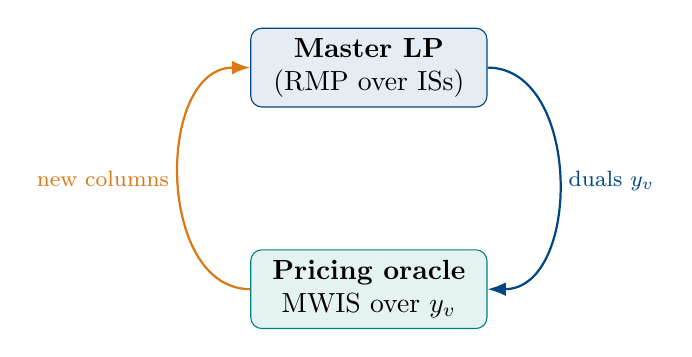
\begin{tikzpicture}[node distance=0.7cm,
                          box/.style={rectangle,rounded corners,
                                      draw=qciblue,fill=qciblue!10,
                                      minimum width=3cm,minimum height=1cm,
                                      align=center},
                          arr/.style={-Latex,qciblue,thick}]
        \node[box] (master) {\textbf{Master LP}\\(RMP over ISs)};
        \node[box,below=1.8cm of master,fill=qciteal!10,draw=qciteal]
          (pricing) {\textbf{Pricing oracle}\\MWIS over $y_v$};
        \draw[arr] (master.east) .. controls +(1.2,0) and +(1.2,0) ..
                   node[midway,right,align=left,font=\footnotesize,yshift=-0.1em]
                   {duals $y_v$} (pricing.east);
        \draw[arr,qciorange] (pricing.west) .. controls +(-1.2,0) and +(-1.2,0) ..
                   node[midway,left,align=right,font=\footnotesize]
                   {new columns} (master.west);
      \end{tikzpicture}
    \end{column}
  \end{columns}
\end{frame}

\begin{frame}{The pricing subproblem is where pricing oracles compete}
  \begin{block}{Key observation}
    On a fixed $(G, y)$ the PSP is NP-hard as MWIS. Any oracle that returns
    profitable ISs works. \textbf{The more columns per call, the fewer master
    solves needed to close the LP.}
  \end{block}

  Two oracles, same PSP interface:
  \begin{itemize}
    \item \lpname: solve MWIS LP relaxation with \texttt{scipy.linprog},
          multi-threshold support extraction + random pruning.
    \item \diracname: submit Motzkin--Straus QP to Dirac-3; 100 raw samples;
          multi-threshold / multi-prune / randomized rounding post-processing.
  \end{itemize}
\end{frame}

% ===========================================================================
\section{Branch-and-Price}

\begin{frame}{Branch-and-Bound tree over colorings}
  \centering
  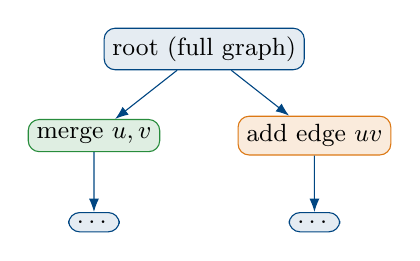
\begin{tikzpicture}[
      level distance=1.1cm,
      sibling distance=2.8cm,
      every node/.style={rectangle,rounded corners,
                         draw=qciblue,fill=qciblue!10,inner sep=3pt,font=\small},
      edge from parent/.style={draw=qciblue,-Latex}]
    \node {root (full graph)}
      child { node [fill=qcigreen!15,draw=qcigreen] {merge $u,v$}
        child { node {\dots} } }
      child { node [fill=qciorange!15,draw=qciorange] {add edge $uv$}
        child { node {\dots} } };
  \end{tikzpicture}
  \vspace{0.5em}
  \begin{itemize}\small
    \item Each node runs its own CG loop on a \emph{modified} graph.
    \item Ryan--Foster binary branching: \textcolor{qcigreen}{merge} (same color) or
          \textcolor{qciorange}{add edge} (different colors) on a fractional pair.
    \item The PSP changes as the graph is modified --- new subproblems to price.
  \end{itemize}
\end{frame}

\begin{frame}{Two branching rules in this repo}
  \begin{description}
    \item[IS-fixing (ISF)] single-child path tree --- fix one IS per level, shrink
          the remaining graph. Original paper method. Cheap but weak lower bound.
    \item[Ryan--Foster (RF)] binary tree on a fractional pair $(u,v)$: left
          merges them, right adds the edge. Monotone LP lower bound; can
          \bestval{prove optimality} when the tree is exhausted.
  \end{description}
\end{frame}

% ===========================================================================
\section{Dirac pricing}

\begin{frame}{Motzkin--Straus for MWIS}
  \begin{columns}[T]
    \begin{column}{0.55\textwidth}
      The weighted Motzkin--Straus trick reformulates max-weight IS as a
      quadratic program on the simplex:
      \[
      \max_{x \ge 0,\,\mathbf{1}^{\!\top}\!x=1} \sum_v w_v x_v^{\,2} \;-\;
      \sum_{(u,v) \in E} x_u x_v
      \]
      Dirac-3 \textbf{directly supports} this primitive:
      $\min\, x^{\top} C + x^{\top} J x$ with $C=0$, $J$ = graph matrix.
      \begin{itemize}\small
        \item Returns \texttt{num\_samples}=100 real vectors of length $|V|$.
        \item Post-processing extracts profitable ISs from these vectors.
      \end{itemize}
    \end{column}
    \begin{column}{0.45\textwidth}
      \centering
      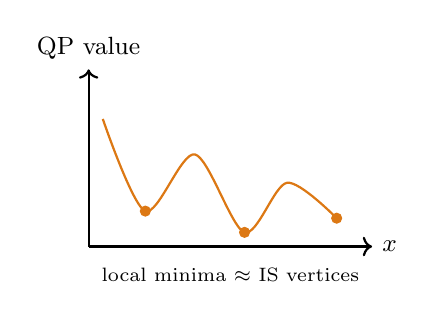
\begin{tikzpicture}[scale=0.9]
        \draw[->,thick] (0,0) -- (4,0) node[right,font=\small] {$x$};
        \draw[->,thick] (0,0) -- (0,2.5) node[above,font=\small] {QP value};
        \draw[qciorange,thick,smooth] plot coordinates
          {(0.2,1.8) (0.8,0.5) (1.5,1.3) (2.2,0.2) (2.8,0.9) (3.5,0.4)};
        \foreach \x/\y in {0.8/0.5, 2.2/0.2, 3.5/0.4}
          \filldraw[qciorange] (\x,\y) circle (2pt);
        \node[font=\scriptsize] at (2,-0.4) {local minima $\approx$ IS vertices};
      \end{tikzpicture}
    \end{column}
  \end{columns}
\end{frame}

\begin{frame}{Dirac's raw response, post-processed into columns}
  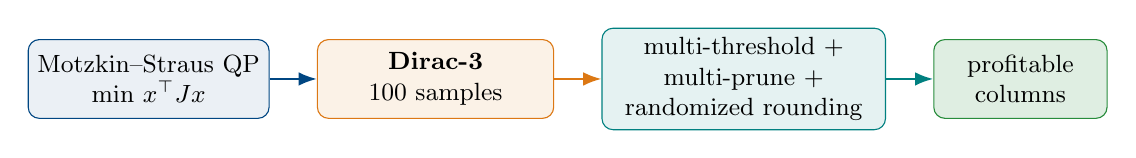
\begin{tikzpicture}[node distance=0.6cm and 0.3cm]
    \node[draw=qciblue,fill=qciblue!8,rounded corners,minimum width=2.4cm,
          minimum height=1cm,align=center,font=\small] (qp)
      {Motzkin--Straus QP\\$\min\,x^{\top}Jx$};
    \node[draw=qciorange,fill=qciorange!10,rounded corners,minimum width=3cm,
          right=0.6cm of qp,minimum height=1cm,align=center,font=\small] (dirac)
      {\textbf{Dirac-3}\\100 samples};
    \node[draw=qciteal,fill=qciteal!10,rounded corners,minimum width=3.6cm,
          right=0.6cm of dirac,minimum height=1cm,align=center,font=\small] (post)
      {multi-threshold +\\multi-prune +\\randomized rounding};
    \node[draw=qcigreen,fill=qcigreen!15,rounded corners,minimum width=2.2cm,
          right=0.6cm of post,minimum height=1cm,align=center,font=\small] (cols)
      {profitable\\columns};
    \draw[-Latex,qciblue,thick] (qp) -- (dirac);
    \draw[-Latex,qciorange,thick] (dirac) -- (post);
    \draw[-Latex,qciteal,thick] (post) -- (cols);
  \end{tikzpicture}
  \vspace{0.8em}
  \begin{itemize}\small
    \item Each sample is a continuous vector of length $|V|$.
    \item Thresholds $\{0.005, 0.01, 0.05, 0.1, 0.2\}$ extract support sets.
    \item Pruning strategies + local search turn each support into a valid IS.
  \end{itemize}
\end{frame}

% ===========================================================================
\section{Zoom-in: CG on ER(20, 0.7)}

\begin{frame}{Pick two pricing subproblems from the QCG run}
  \begin{center}
    On ER(20, 0.7): QCG runs 6 pricing calls. We compare the \diracname{} vs
    \lpname{} outputs on two representative PSPs:
    \vspace{0.8em}

    \begin{tabular}{l l l}
      \toprule
      \textbf{PSP \#1} & call\_00 & uniform duals $y_v = 1/\chi$\\
      \textbf{PSP \#2} & call\_03 & differentiated duals (mid CG iter)\\
      \bottomrule
    \end{tabular}
  \end{center}
\end{frame}

% --- PSP #1 ---------------------------------------------------------------
\begin{frame}{PSP \#1: dual weights (uniform, first CG iter)}
  \begin{center}
    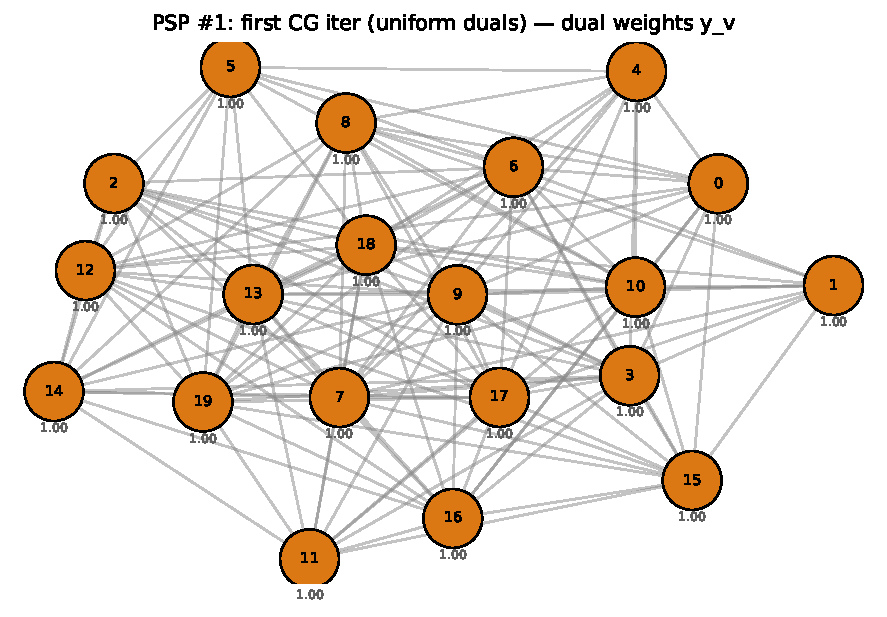
\includegraphics[width=0.58\textwidth]{figures/05_psp01_duals.pdf}\\[0.4em]
    \small All $y_v$ equal $\approx$ 0.13 --- the PSP is effectively unweighted MWIS.
  \end{center}
\end{frame}

\begin{frame}{PSP \#1: LP pricing columns ($16$)}
  \begin{center}
    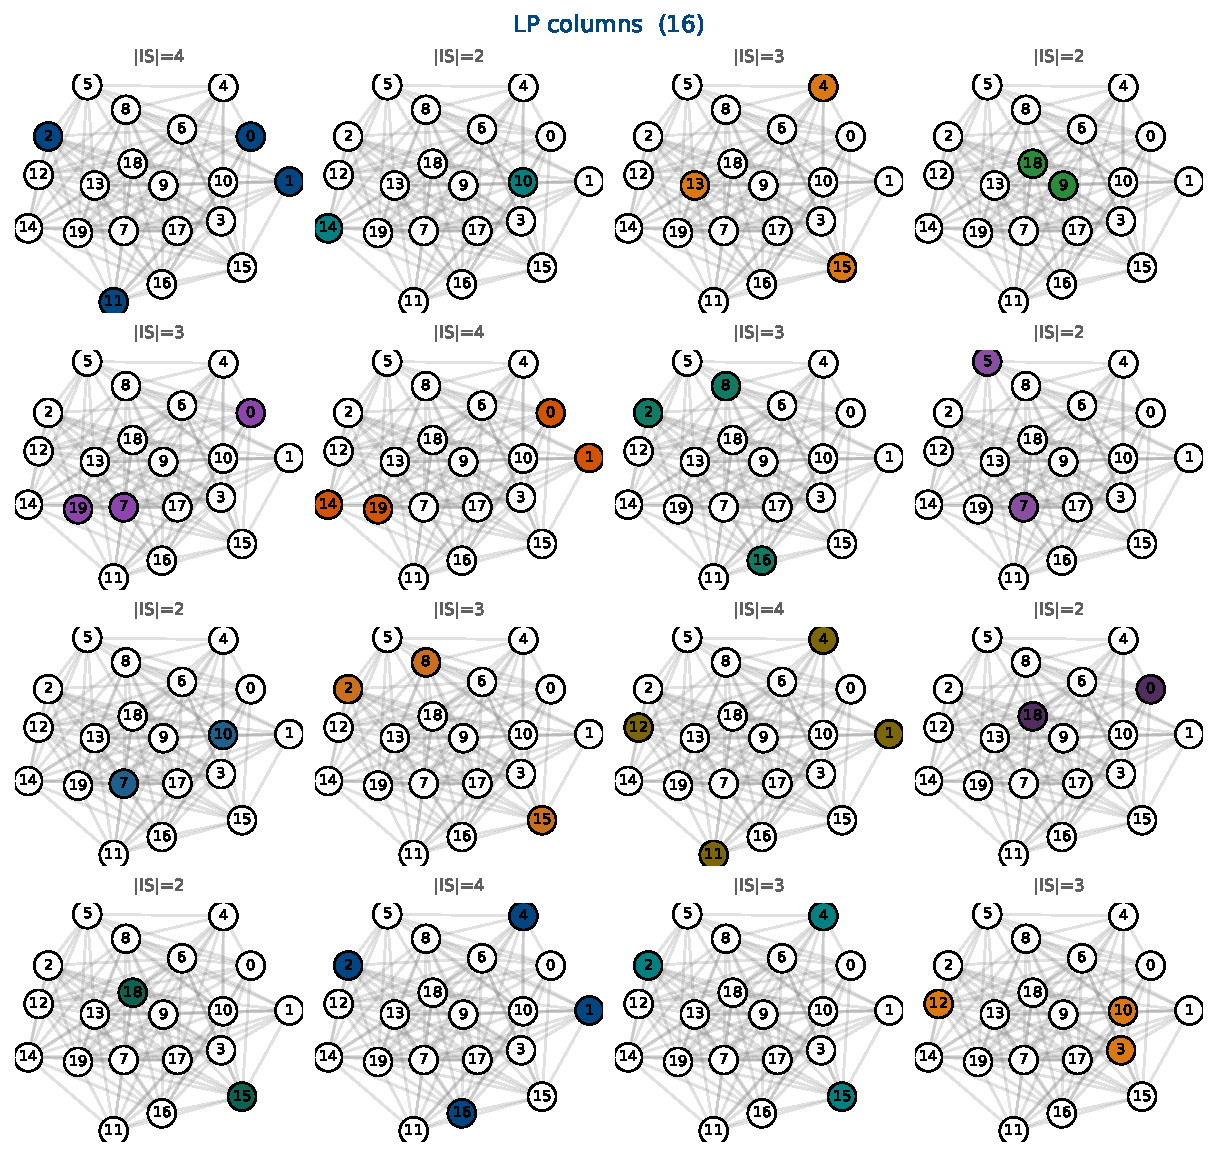
\includegraphics[width=0.98\textwidth]{figures/05_psp01_lp_cols.pdf}
  \end{center}
\end{frame}

\begin{frame}{PSP \#1: Dirac pricing columns ($4$)}
  \begin{center}
    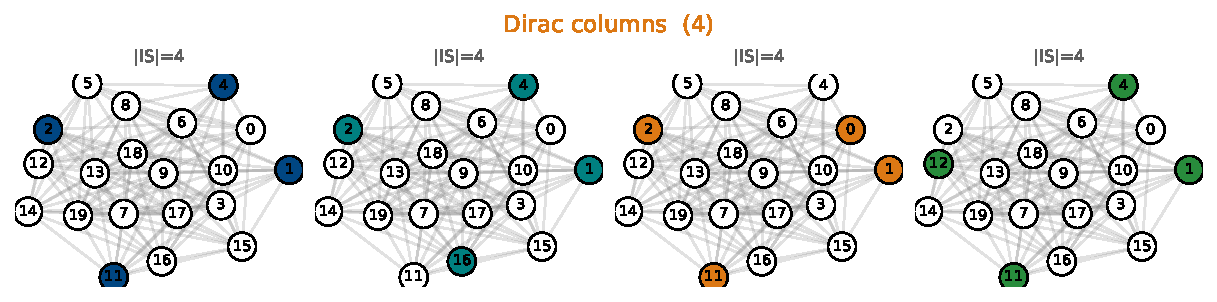
\includegraphics[width=0.98\textwidth]{figures/05_psp01_dirac_cols.pdf}
  \end{center}
\end{frame}

\begin{frame}{PSP \#1: stats}
  \begin{center}
    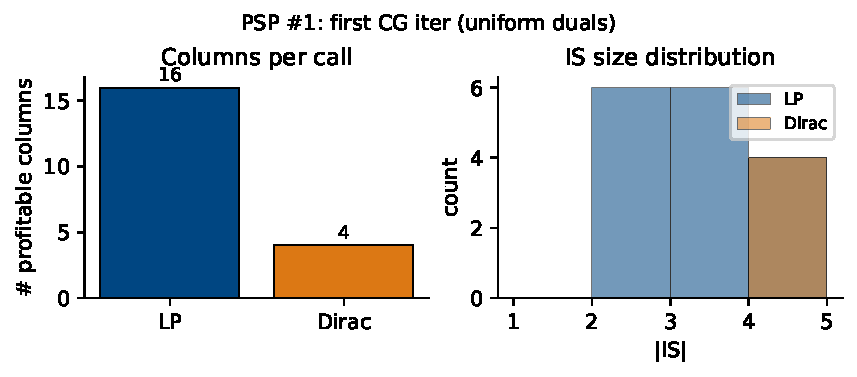
\includegraphics[width=0.8\textwidth]{figures/05_psp01_stats.pdf}
  \end{center}
  \small
  On uniform duals, the LP returns an \emph{integral-ish} polytope vertex from
  which many support-threshold variants expose distinct maximum ISs. Dirac's
  samples spread (no direction) and the extractor finds fewer.
\end{frame}

% --- PSP #2 ---------------------------------------------------------------
\begin{frame}{PSP \#2: dual weights (differentiated, mid CG iter)}
  \begin{center}
    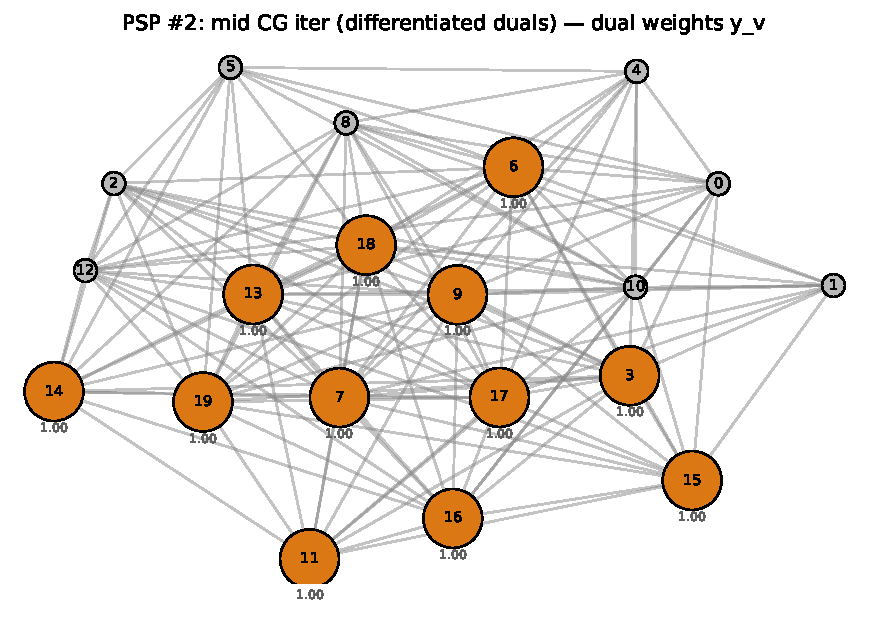
\includegraphics[width=0.58\textwidth]{figures/06_psp02_duals.pdf}\\[0.4em]
    \small After 3 CG iterations the LP concentrates weight on hard-to-cover vertices;
    8 vertices have been filtered out (grey).
  \end{center}
\end{frame}

\begin{frame}{PSP \#2: LP pricing columns}
  \begin{center}
    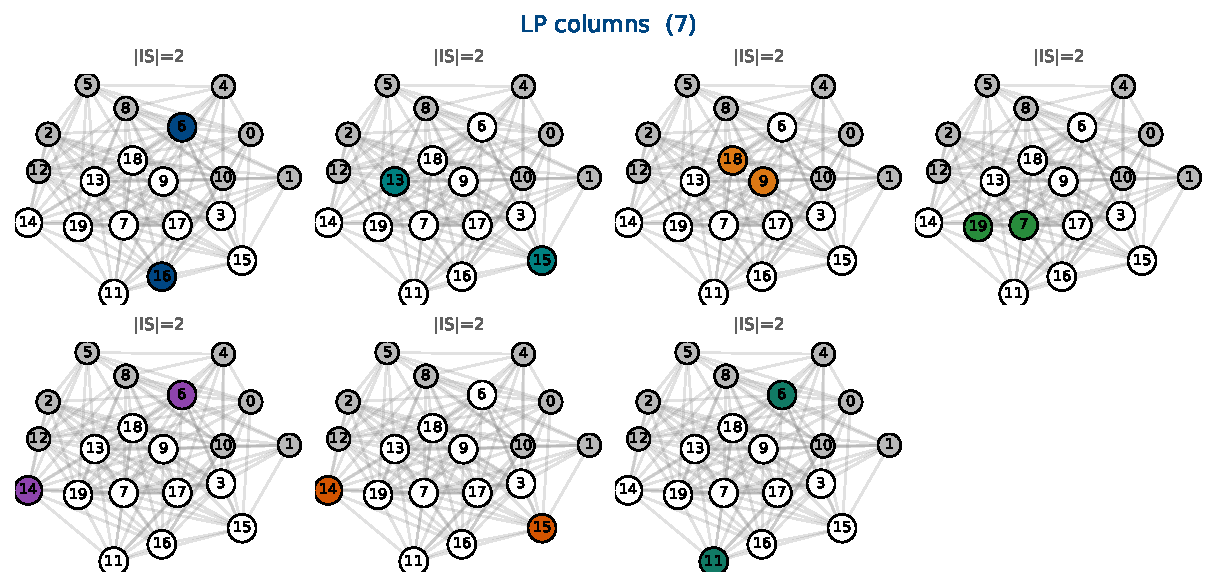
\includegraphics[width=0.98\textwidth]{figures/06_psp02_lp_cols.pdf}
  \end{center}
\end{frame}

\begin{frame}{PSP \#2: Dirac pricing columns}
  \begin{center}
    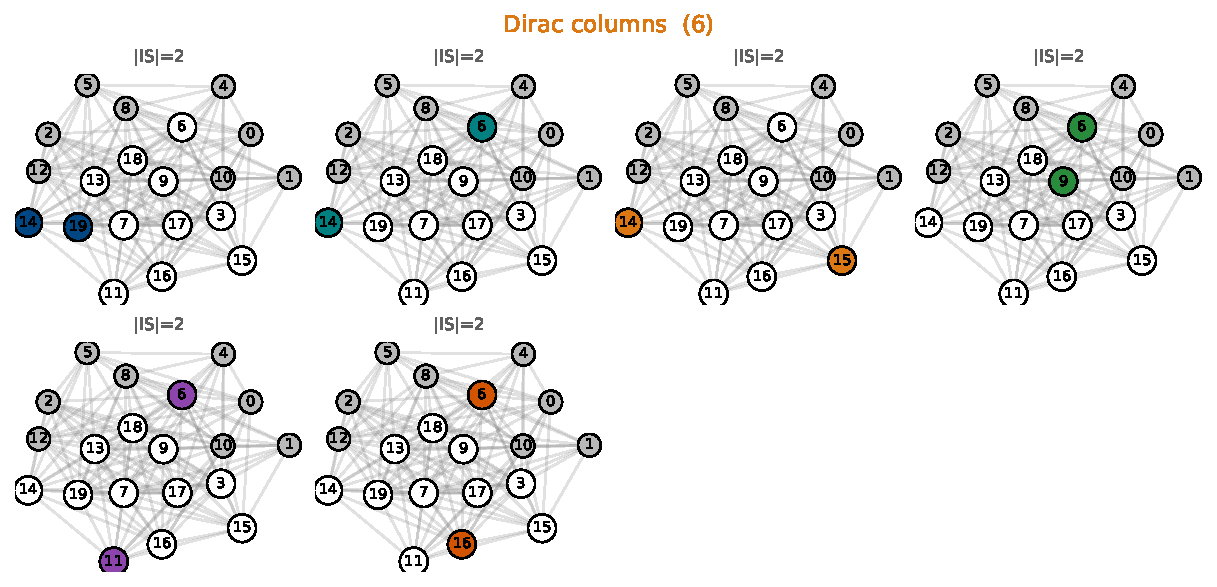
\includegraphics[width=0.98\textwidth]{figures/06_psp02_dirac_cols.pdf}
  \end{center}
\end{frame}

\begin{frame}{PSP \#2: stats}
  \begin{center}
    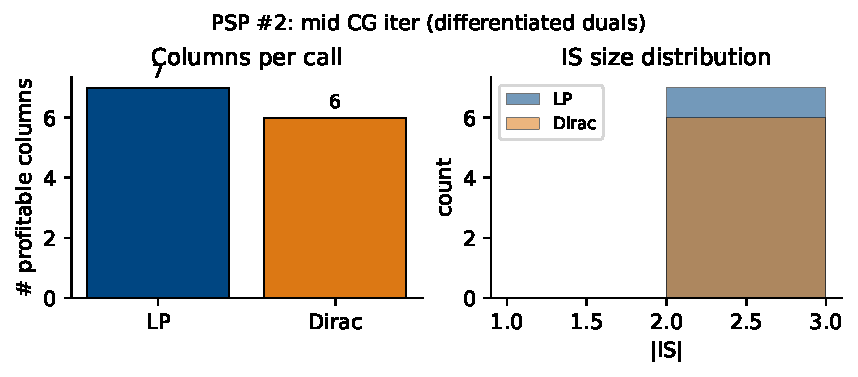
\includegraphics[width=0.8\textwidth]{figures/06_psp02_stats.pdf}
  \end{center}
\end{frame}

% ===========================================================================
\section{Summary}

\begin{frame}{Columns-per-call: aggregate view across the benchmark suite}
  \begin{center}
    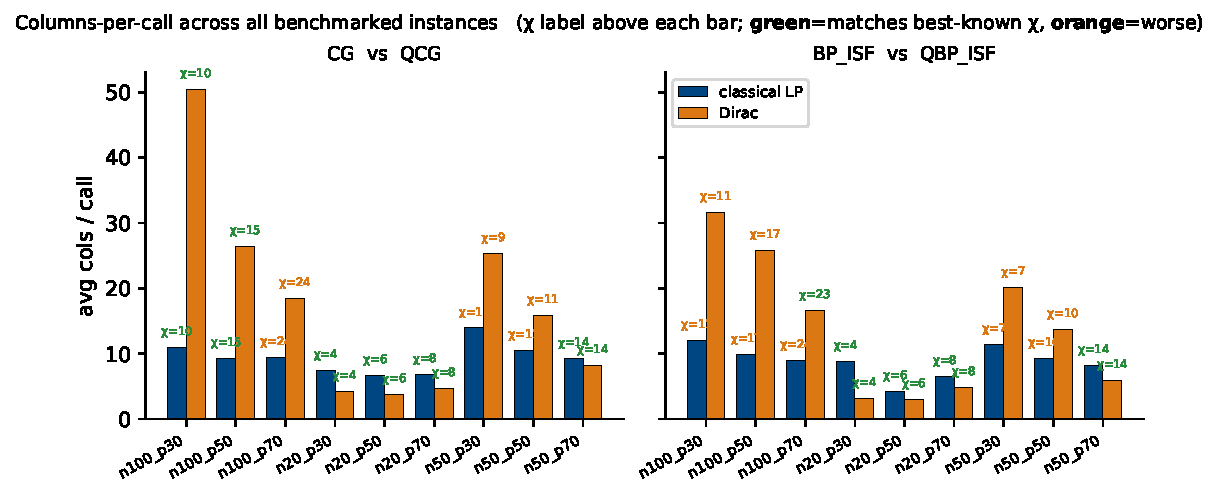
\includegraphics[width=0.98\textwidth]{figures/09_summary_bars.pdf}
  \end{center}
\end{frame}

\begin{frame}{Iterations to solution}
  \begin{center}
    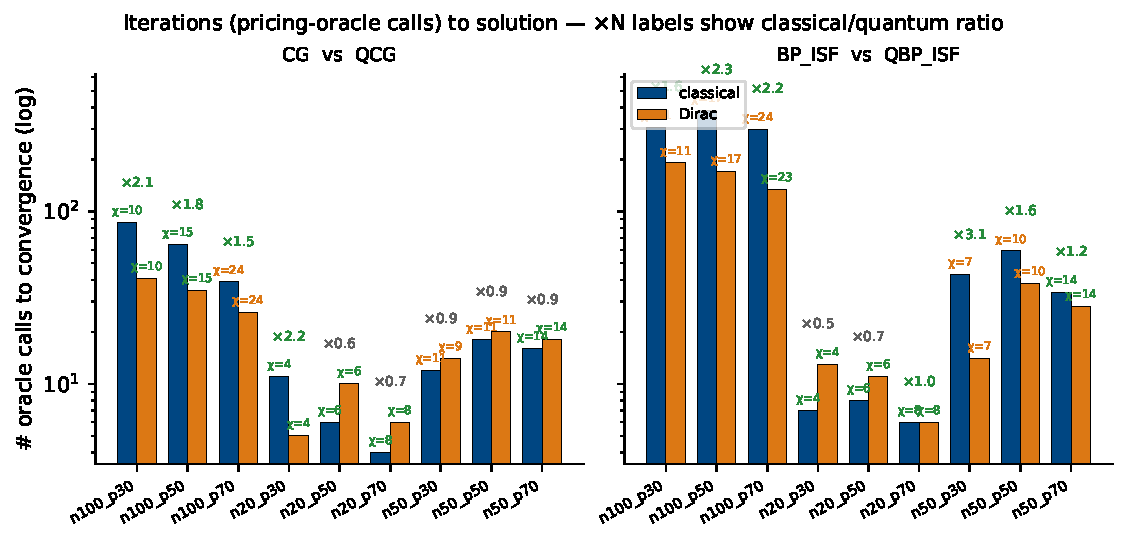
\includegraphics[width=0.98\textwidth]{figures/10_iterations_bars.pdf}\\[0.3em]
    \small Fewer pricing-oracle calls close the LP / B\&P tree.
    \textcolor{qcigreen}{$\times\!N$} labels show the classical-to-Dirac ratio
    (\bestval{higher = Dirac converges in fewer calls}).
  \end{center}
\end{frame}

\begin{frame}{Branch-and-Bound tree size (IS-fixing)}
  \begin{center}
    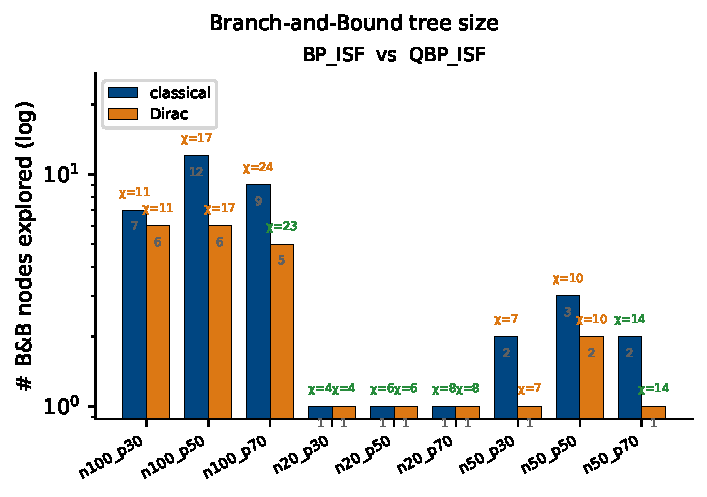
\includegraphics[width=0.55\textwidth]{figures/11_bp_nodes_bars.pdf}\\[0.4em]
    \small QBP-ISF closes the tree with \bestval{fewer or equal B\&B nodes}
    than classical BP-ISF on the n\,=\,100 instances, consistent with
    Dirac's richer column pool per call.
  \end{center}
\end{frame}

\begin{frame}{Full benchmark table}
  \vspace{-0.2em}
  \scriptsize
  % Auto-generated by pipeline/render_figures.py — do not edit.
\renewcommand{\arraystretch}{1.05}
\begin{tabular}{@{}l cc cccc@{}}
\toprule
 & \multicolumn{2}{c}{reference} & \multicolumn{4}{c}{pricing method: $\chi$ (iters / cols-per-call)} \\
\cmidrule(lr){2-3}\cmidrule(lr){4-7}
Instance & MILP & Hexaly & CG & QCG & BP-ISF & QBP-ISF \\
\midrule
$n{=}20$, $p{=}0.3$ & \bestval{4}\cmark & \bestval{4}\cmark & \bestval{4} (11/7.5) & \bestval{4} (5/4.2) & \bestval{4}\cmark (7/8.9) & \bestval{4}\cmark (13/3.1) \\
$n{=}20$, $p{=}0.5$ & \bestval{6}\cmark & \bestval{6}\cmark & \bestval{6} (6/6.7) & \bestval{6} (10/3.7) & \bestval{6}\cmark (8/4.2) & \bestval{6}\cmark (11/3.0) \\
$n{=}20$, $p{=}0.7$ & \bestval{8}\cmark & \bestval{8}\cmark & \bestval{8} (4/6.8) & \bestval{8} (6/4.7) & \bestval{8}\cmark (6/6.5) & \bestval{8}\cmark (6/4.8) \\
$n{=}50$, $p{=}0.3$ & \bestval{6}\cmark & \bestval{6}\cmark & 11 (12/13.9) & 9 (14/25.3) & 7 (43/11.4) & 7\cmark (14/20.1) \\
$n{=}50$, $p{=}0.5$ & \bestval{9} & \bestval{9} & 11 (18/10.5) & 11 (20/15.8) & 10 (59/9.2) & 10 (38/13.7) \\
$n{=}50$, $p{=}0.7$ & \bestval{14} & \bestval{14} & \bestval{14} (16/9.2) & \bestval{14} (18/8.2) & \bestval{14}\cmark (34/8.2) & \bestval{14}\cmark (28/5.9) \\
$n{=}100$, $p{=}0.3$ & \bestval{10} & \bestval{10} & \bestval{10} (86/11.0) & \bestval{10} (41/50.5) & 11 (308/12.0) & 11 (191/31.7) \\
$n{=}100$, $p{=}0.5$ & 17 & 17 & \bestval{15} (64/9.3) & \bestval{15} (35/26.5) & 17 (386/9.8) & 17 (170/25.9) \\
$n{=}100$, $p{=}0.7$ & 28 & \bestval{23} & 24 (39/9.4) & 24 (26/18.4) & 24 (300/8.9) & \bestval{23} (134/16.5) \\
\bottomrule
\end{tabular}

  \vspace{0.4em}

  \scriptsize
  \bestval{bold} = matches the best-known $\chi$ for that instance;
  \cmark = method proves optimality.
  ``$\chi$ (iters / cpc)'' reports chromatic number / oracle calls / avg columns per call.
  For n=100 p=0.3, 0.5 the final set-cover ILP initially timed out on the
  large replayed column pool with HiGHS; re-solving with \textbf{Hexaly}
  (600\,s cap) recovers \textbf{$\chi=10$} (p=0.3) and \textbf{$\chi=15$}
  (p=0.5).
\end{frame}

\begin{frame}{Takeaways}
  \begin{itemize}
    \item At \textbf{small $n$} (n=20) and early CG iterations, \lpname{}
          extraction is competitive or better --- integral LP vertices
          expose multiple ISs through simple thresholding.
    \item At \textbf{large $n$} (n=100), \diracname{} wins both
          \bestval{cols-per-call} (2--4$\times$) and
          \bestval{iterations-to-solution} (1.5--2.3$\times$ fewer
          oracle calls for CG and IS-fixing B\&P). Sample diversity from
          100 raw solutions dominates LP's deterministic polytope vertex.
    \item \textcolor{qciorange}{Per-call latency} on Dirac
          ($\sim$\,50\,s device + queue) shifts the advantage into
          \emph{call count}, not \emph{wall seconds}. For time-to-solution,
          classical remains faster on these instances.
    \item All raw Dirac samples and LP primal vectors are persisted for
          offline post-processing ablations --- no new API calls needed.
  \end{itemize}
\end{frame}

\end{document}
